\documentclass[a4paper,titlepage]{article}
\usepackage[top=1in, bottom=1.25in, left=1.25in, right=1.25in]{geometry}

\parskip=10pt

\usepackage[scaled]{beramono}
\usepackage[T1]{fontenc}

\usepackage{amsmath}

\usepackage{listings}
\lstset{basicstyle=\footnotesize\ttfamily,tabsize=4,breaklines,frame=single, moredelim=[is][\underbar]{__}{__}}

\usepackage{graphicx}
\usepackage{tikz}
\usepackage{float}
\usepackage{booktabs}

\renewcommand{\figurename}{Gambar}
\renewcommand{\refname}{Referensi}

\begin{document}

	\title{Laporan Tugas I \\ IF2220 Teori Bahasa Formal dan Automata}
	\author{Jonathan Christopher / 13515001 / K-01}
	\maketitle

	\section{Deskripsi Persoalan}

		Persoalan yang harus diselesaikan dalam tugas ini adalah membuat sebuah program yang dapat menerima dan menjalankan sebuah \textit{deterministic finite state automata} (DFA) yang didefinisikan dalam sebuah file terpisah. Program tersebut harus dapat membaca definisi DFA yang terkandung dalam sebuah file eksternal, antara lain daftar \textit{state}, alfabet/daftar simbol masukan, fungsi transisi, serta \textit{state-state} awal dan akhir. Program kemudian akan menerima sebuah \textit{string} input untuk dijalankan pada DFA tersebut. Berdasarkan \textit{string} tersebut, program kemudian harus menampilkan urutan \textit{state-state} yang dilewati, serta apakah \textit{string} tersebut diterima oleh DFA yang sedang dipakai (\textit{state} paling akhir harus merupakan sebuah \textit{final/accepting state}).

		DFA yang harus dibuat didasarkan pada soal 2.2.1 di buku \textit{Introduction to Automata Theory, Languages and Computation}. DFA tersebut merepresentasikan sebuah mesin kelereng yang memiliki beberapa jalur yang dapat dilalui, serta tiga buah tuas yang berubah arah setiap kali setelah dilalui oleh kelereng. Simbol input dari mesin ini adalah slot tempat kelereng dimasukkan, yaitu slot A atau B. Kelereng juga dapat keluar melalui jalur C atau D. Jika kelereng terakhir yang dimasukkan keluar melalui jalur D, maka input diterima; sedangkan bila kelereng terakhir keluar melalui jalur C atau belum ada kelereng yang dimasukkan, input tidak diterima.

		\begin{figure}[h]
		    \centering
		    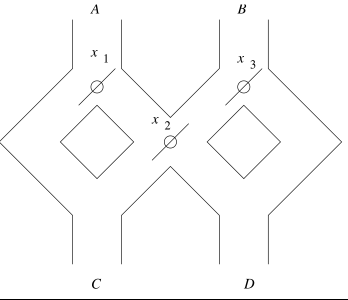
\includegraphics[width=0.5\textwidth]{marble.png}
		    \caption{Mesin kelereng pada \textit{Exercise 2.2.1}}
		    \label{fig:marble}
		\end{figure}

	\section{\textit{Deterministic Finite Automata}}

		\textit{Deterministic finite automata} yang digunakan untuk merepresentasikan mesin kelereng pada persoalan ini adalah:
		\[A = (Q, \Sigma, \delta, q_0, F)\]
		dengan
		\begin{equation*}
			\begin{split}
				Q = \{ & LLLC, RLLC, LRRC, LRLC, RRRC, LRLD, RRLC, LLRD, \\
					& RRLD, LLLD, RLRD, RLRC, RLLD\}
			\end{split}
		\end{equation*}
		\[\Sigma = \{A, B\}\]
		\[q_0 = LLLC\]
		\[F = \{LRLD, LLRD, RRLD, LLLD, RLRD, RLLD\}\]
		dan fungsi transisi yang didefinisikan sebagai berikut:
		\[
			\delta(q, a) = \left\{
				\begin{array}{lr}
					RLLC, & q = LLLC \text{ dan } a = A\\
					LRRC, & q = LLLC \text{ dan } a = B\\
					LRLC, & q = RLLC \text{ dan } a = A\\
					RRRC, & q = RLLC \text{ dan } a = B\\
					RRRC, & q = LRRC \text{ dan } a = A\\
					LRLD, & q = LRRC \text{ dan } a = B\\
					RRLC, & q = LRLC \text{ dan } a = A\\
					LLRD, & q = LRLC \text{ dan } a = B\\
					LLRD, & q = RRRC \text{ dan } a = A\\
					RRLD, & q = RRRC \text{ dan } a = B\\
					RRLC, & q = LRLD \text{ dan } a = A\\
					LLRD, & q = LRLD \text{ dan } a = B\\
					LLLD, & q = RRLC \text{ dan } a = A\\
					RLRD, & q = RRLC \text{ dan } a = B\\
					RLRC, & q = LLRD \text{ dan } a = A\\
					LLLD, & q = LLRD \text{ dan } a = B\\
					LLLD, & q = RRLD \text{ dan } a = A\\
					RLRD, & q = RRLD \text{ dan } a = B\\
					RLLC, & q = LLLD \text{ dan } a = A\\
					LRRC, & q = LLLD \text{ dan } a = B\\
					LRRC, & q = RLRD \text{ dan } a = A\\
					RLLD, & q = RLRD \text{ dan } a = B\\
					LRRC, & q = RLRC \text{ dan } a = A\\
					RLLD, & q = RLRC \text{ dan } a = B\\
					LRLC, & q = RLLD \text{ dan } a = A\\
					RRRC, & q = RLLD \text{ dan } a = B
				\end{array}
			\right\}
		\]

		Karakter-karakter pada nama \textit{state} secara berturut-turut melambangkan posisi tuas $x_1$, $x_2$, dan $x_3$, serta jalur terakhir yang dilewati oleh kelereng (C atau D). Jika belum ada kelereng yang lewat, dianggap nilai jalur terakhir tersebut bernilai C karena keadaan tersebut juga tidak diterima oleh DFA.

		\begin{table}[H]
			\centering
			\begin{tabular}{@{}rlcc@{}}
				\toprule
				              &      & A    & B    \\ \midrule
				$\rightarrow$ & LLLC & RLLC & LRRC \\
				              & RLLC & LRLC & RRRC \\
				              & LRRC & RRRC & LRLD \\
				              & LRLC & RRLC & LLRD \\
				              & RRRC & LLRD & RRLD \\
				$\ast$        & LRLD & RRLC & LLRD \\
				              & RRLC & LLLD & RLRD \\
				$\ast$        & LLRD & RLRC & LLLD \\
				$\ast$        & RRLD & LLLD & RLRD \\
				$\ast$        & LLLD & RLLC & LRRC \\
				$\ast$        & RLRD & LRRC & RLLD \\
				              & RLRC & LRRC & RLLD \\
				$\ast$        & RLLD & LRLC & RRRC \\ \bottomrule
			\end{tabular}
			\caption{Tabel transisi untuk DFA mesin kelereng}
			\label{tab:marbledfa}
		\end{table}

		\begin{figure}[H]
			\centering
			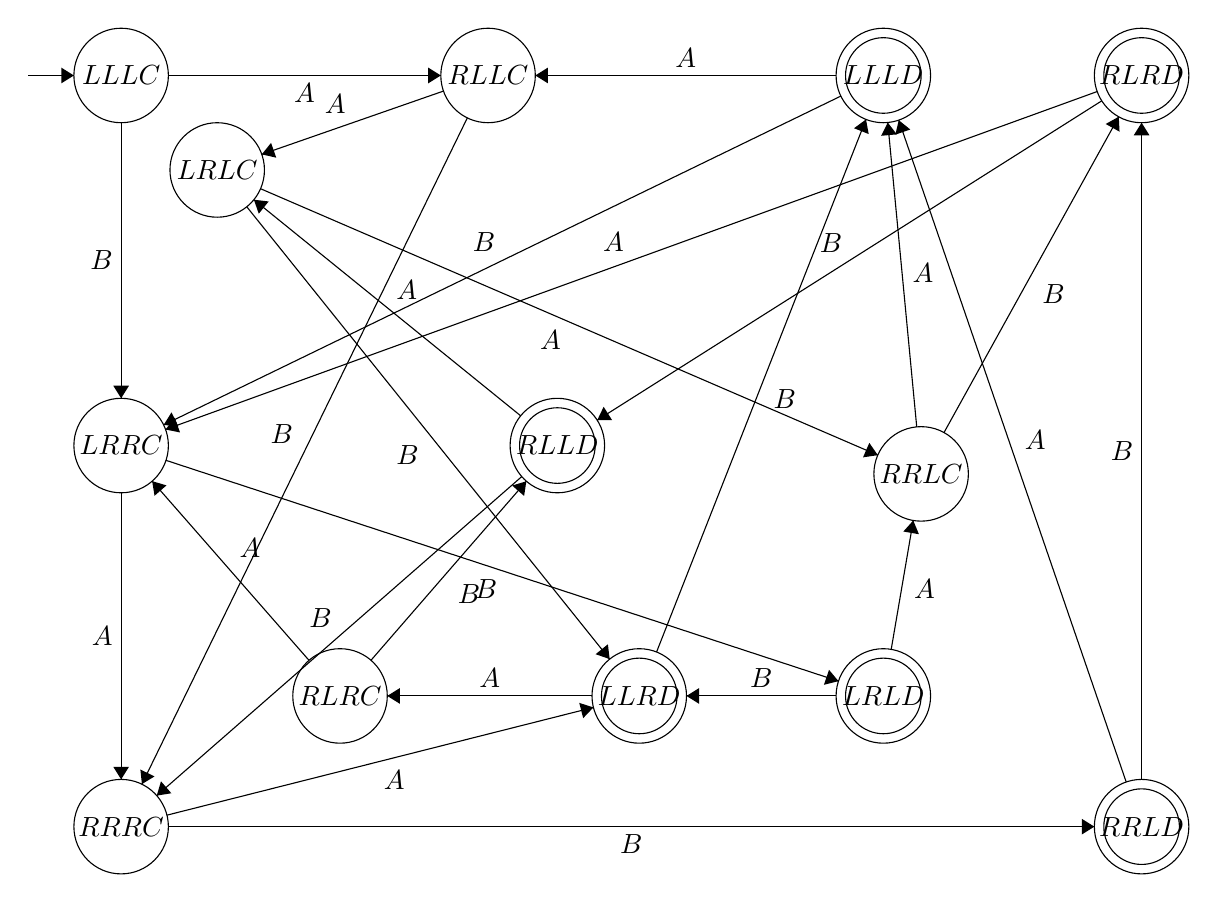
\begin{tikzpicture}[scale=0.2]
				\tikzstyle{every node}+=[inner sep=0pt]
				\draw [black] (7.8,-5.4) circle (3);
				\draw (7.8,-5.4) node {$LLLC$};
				\draw [black] (13.9,-11.4) circle (3);
				\draw (13.9,-11.4) node {$LRLC$};
				\draw [black] (7.8,-53.1) circle (3);
				\draw (7.8,-53.1) node {$RRRC$};
				\draw [black] (31.1,-5.4) circle (3);
				\draw (31.1,-5.4) node {$RLLC$};
				\draw [black] (56.2,-44.8) circle (3);
				\draw (56.2,-44.8) node {$LRLD$};
				\draw [black] (56.2,-44.8) circle (2.4);
				\draw [black] (7.8,-28.9) circle (3);
				\draw (7.8,-28.9) node {$LRRC$};
				\draw [black] (58.6,-30.7) circle (3);
				\draw (58.6,-30.7) node {$RRLC$};
				\draw [black] (40.7,-44.8) circle (3);
				\draw (40.7,-44.8) node {$LLRD$};
				\draw [black] (40.7,-44.8) circle (2.4);
				\draw [black] (72.6,-53.1) circle (3);
				\draw (72.6,-53.1) node {$RRLD$};
				\draw [black] (72.6,-53.1) circle (2.4);
				\draw [black] (56.2,-5.4) circle (3);
				\draw (56.2,-5.4) node {$LLLD$};
				\draw [black] (56.2,-5.4) circle (2.4);
				\draw [black] (72.6,-5.4) circle (3);
				\draw (72.6,-5.4) node {$RLRD$};
				\draw [black] (72.6,-5.4) circle (2.4);
				\draw [black] (21.7,-44.8) circle (3);
				\draw (21.7,-44.8) node {$RLRC$};
				\draw [black] (35.5,-28.9) circle (3);
				\draw (35.5,-28.9) node {$RLLD$};
				\draw [black] (35.5,-28.9) circle (2.4);
				\draw [black] (10.8,-5.4) -- (28.1,-5.4);
				\fill [black] (28.1,-5.4) -- (27.3,-4.9) -- (27.3,-5.9);
				\draw (19.45,-5.9) node [below] {$A$};
				\draw [black] (7.8,-8.4) -- (7.8,-25.9);
				\fill [black] (7.8,-25.9) -- (8.3,-25.1) -- (7.3,-25.1);
				\draw (7.3,-17.15) node [left] {$B$};
				\draw [black] (28.27,-6.39) -- (16.73,-10.41);
				\fill [black] (16.73,-10.41) -- (17.65,-10.62) -- (17.32,-9.68);
				\draw (21.39,-7.86) node [above] {$A$};
				\draw [black] (29.78,-8.1) -- (9.12,-50.4);
				\fill [black] (9.12,-50.4) -- (9.92,-49.91) -- (9.02,-49.47);
				\draw (18.75,-28.17) node [left] {$B$};
				\draw [black] (7.8,-31.9) -- (7.8,-50.1);
				\fill [black] (7.8,-50.1) -- (8.3,-49.3) -- (7.3,-49.3);
				\draw (7.3,-41) node [left] {$A$};
				\draw [black] (10.65,-29.84) -- (53.35,-43.86);
				\fill [black] (53.35,-43.86) -- (52.75,-43.14) -- (52.43,-44.09);
				\draw (30.97,-37.39) node [below] {$B$};
				\draw [black] (15.78,-13.74) -- (38.82,-42.46);
				\fill [black] (38.82,-42.46) -- (38.71,-41.52) -- (37.93,-42.15);
				\draw (26.74,-29.52) node [left] {$B$};
				\draw [black] (10.71,-52.37) -- (37.79,-45.53);
				\fill [black] (37.79,-45.53) -- (36.89,-45.24) -- (37.14,-46.21);
				\draw (25.14,-49.53) node [below] {$A$};
				\draw [black] (10.8,-53.1) -- (69.6,-53.1);
				\fill [black] (69.6,-53.1) -- (68.8,-52.6) -- (68.8,-53.6);
				\draw (40.2,-53.6) node [below] {$B$};
				\draw [black] (56.7,-41.84) -- (58.1,-33.66);
				\fill [black] (58.1,-33.66) -- (57.47,-34.36) -- (58.46,-34.53);
				\draw (58.12,-37.99) node [right] {$A$};
				\draw [black] (53.2,-44.8) -- (43.7,-44.8);
				\fill [black] (43.7,-44.8) -- (44.5,-45.3) -- (44.5,-44.3);
				\draw (48.45,-44.3) node [above] {$B$};
				\draw [black] (58.32,-27.71) -- (56.48,-8.39);
				\fill [black] (56.48,-8.39) -- (56.06,-9.23) -- (57.06,-9.14);
				\draw (58.03,-17.97) node [right] {$A$};
				\draw [black] (60.05,-28.08) -- (71.15,-8.02);
				\fill [black] (71.15,-8.02) -- (70.32,-8.48) -- (71.2,-8.97);
				\draw (66.27,-19.25) node [right] {$B$};
				\draw [black] (37.7,-44.8) -- (24.7,-44.8);
				\fill [black] (24.7,-44.8) -- (25.5,-45.3) -- (25.5,-44.3);
				\draw (31.2,-44.3) node [above] {$A$};
				\draw [black] (41.8,-42.01) -- (55.1,-8.19);
				\fill [black] (55.1,-8.19) -- (54.34,-8.75) -- (55.27,-9.12);
				\draw (49.2,-25.97) node [right] {$B$};
				\draw [black] (71.62,-50.26) -- (57.18,-8.24);
				\fill [black] (57.18,-8.24) -- (56.96,-9.16) -- (57.91,-8.83);
				\draw (65.16,-28.52) node [right] {$A$};
				\draw [black] (72.6,-50.1) -- (72.6,-8.4);
				\fill [black] (72.6,-8.4) -- (72.1,-9.2) -- (73.1,-9.2);
				\draw (72.1,-29.25) node [left] {$B$};
				\draw [black] (53.2,-5.4) -- (34.1,-5.4);
				\fill [black] (34.1,-5.4) -- (34.9,-5.9) -- (34.9,-4.9);
				\draw (43.65,-4.9) node [above] {$A$};
				\draw [black] (53.5,-6.71) -- (10.5,-27.59);
				\fill [black] (10.5,-27.59) -- (11.44,-27.69) -- (11,-26.79);
				\draw (30.85,-16.64) node [above] {$B$};
				\draw [black] (69.78,-6.42) -- (10.62,-27.88);
				\fill [black] (10.62,-27.88) -- (11.54,-28.07) -- (11.2,-27.13);
				\draw (39.07,-16.62) node [above] {$A$};
				\draw [black] (70.07,-7.01) -- (38.03,-27.29);
				\fill [black] (38.03,-27.29) -- (38.98,-27.29) -- (38.44,-26.44);
				\draw (52.88,-16.65) node [above] {$B$};
				\draw [black] (19.73,-42.54) -- (9.77,-31.16);
				\fill [black] (9.77,-31.16) -- (9.92,-32.09) -- (10.68,-31.43);
				\draw (15.29,-35.4) node [right] {$A$};
				\draw [black] (23.67,-42.53) -- (33.53,-31.17);
				\fill [black] (33.53,-31.17) -- (32.63,-31.44) -- (33.39,-32.1);
				\draw (29.14,-38.3) node [right] {$B$};
				\draw [black] (33.17,-27.01) -- (16.23,-13.29);
				\fill [black] (16.23,-13.29) -- (16.54,-14.18) -- (17.17,-13.4);
				\draw (25.93,-19.66) node [above] {$A$};
				\draw [black] (33.24,-30.87) -- (10.06,-51.13);
				\fill [black] (10.06,-51.13) -- (10.99,-50.98) -- (10.33,-50.22);
				\draw (20.47,-40.51) node [above] {$B$};
				\draw [black] (1.9,-5.4) -- (4.8,-5.4);
				\fill [black] (4.8,-5.4) -- (4,-4.9) -- (4,-5.9);
				\draw [black] (16.65,-12.59) -- (55.85,-29.51);
				\fill [black] (55.85,-29.51) -- (55.31,-28.73) -- (54.91,-29.65);
				\draw (35.06,-21.56) node [below] {$A$};
			\end{tikzpicture}
			\caption{Diagram DFA mesin kelereng}
		    \label{fig:marbledfa}
		\end{figure}

	\section{Daftar Asumsi}

	Asumsi-asumsi yang digunakan dalam penyelesaian persoalan untuk tugas ini adalah:

		\begin{itemize}
			\item Sebuah simbol terdiri atas tepat satu karakter
			\item Batas maksimum jumlah simbol adalah 255 simbol
			\item Nama sebuah \textit{state} adalah sebuah \textit{string} tidak kosong yang tidak mengandung karakter \textit{whitespace} (spasi, \textit{newline} dsb.) dan memiliki panjang maksimum 1023 karakter
			\item Jumlah \textit{state} maksimal yang dapat diproses adalah sekitar $2^{31}-1$ \textit{state}, jika memori sistem tempat program dijalankan memadai
			\item Nama \textit{state} dan simbol bersifat \textit{case-sensitive}
			\item Panjang \textit{file path} relatif yang dimasukkan ke program untuk memilih \textit{file} DFA tidak lebih dari 255 karakter
			\item \textit{String} simbol dalam input pengguna terdiri dari karakter-karakter yang terdefinisi sebagai simbol untuk DFA yang sedang dijalankan, serta memiliki panjang tidak lebih dari 1023 karakter
			\item Jika dalam \textit{string} input pengguna terdapat karakter yang tidak terdefinisi sebagai simbol untuk DFA yang sedang dijalankan, maka karakter tersebut akan dibiarkan dan \textit{state} DFA tidak akan berubah
			\item DFA yang diberikan merupakan DFA yang valid dengan fungsi transisi yang terdefinisi lengkap
			\item \textit{File} DFA pasti valid sesuai format yang telah ditentukan:
		\end{itemize}

		\begin{lstlisting}
<string yang masing-masing karakternya melambangkan sebuah simbol (tidak boleh mengandung whitespace dalam string dan harus unik, maksimal 255 karakter)>

<jumlah state (1 <= n <= 1023)>
<nama-nama state dipisahkan whitespace (isi nama tidak boleh mengandung whitespace dan harus unik, maksimal 1023 karakter)>

<jumlah final state (1 <= n <= jumlah state)>
<nama-nama final state dipisahkan whitespace (harus unik dan harus ada di daftar state)>

<nama state awal (hanya 1, harus ada di daftar state)>

<representasi fungsi transisi dalam bentuk tabel (baris mengacu pada nama state awal (urutan sesuai daftar state), kolom mengacu pada simbol (urutan sesuai daftar simbol), isi merupakan nama state tujuan)>
		\end{lstlisting}

	\section{\textit{Source Code}}

		\subsection{dfa.h}
			\lstinputlisting[language=C]{../src/dfa.h}

		\subsection{dfa.c}
			\lstinputlisting[language=C]{../src/dfa.c}

		\subsection{main.c}
			\lstinputlisting[language=C]{../src/main.c}

		\subsection{marble.dfa}
			\lstinputlisting{../src/marble.dfa}

	\section{Contoh Interaksi dengan Program}

		Berikut adalah contoh interaksi pengguna dengan program. Input pengguna digarisbawahi.

		\begin{lstlisting}
Automaton - Tugas I IF2220 Teori Bahasa Formal dan Automata
===========================================================

NIM       : 13515001
Nama      : Jonathan Christopher
Kelas     : K-01, TBFO IF2220
Tanggal   : 12 September 2016
Topik     : DFA
Deskripsi : Program sederhana untuk mengecek apakah suatu string diterima oleh DFA tertentu, serta contoh DFA berdasarkan Exercise 2.2.1 dari buku Introduction to Automata Theory, Languages, and Computation (3rd ed.)

Path ke file DFA (untuk tugas TBFO, gunakan ../src/marble.dfa): __../src/marble.dfa__
DFA berhasil dibaca.
Simbol-simbol yang diterima: A B

Masukkan input string: __AAAB__
LLLC -> RLLC -> LRLC -> RRLC -> RLRD
String diterima? Ya (berakhir di final state)
Coba lagi? (y/n): __y__

Masukkan input string: __A__
LLLC -> RLLC
String diterima? Tidak (tidak berakhir di final state)
Coba lagi? (y/n): __y__

Masukkan input string: __BBBBBBA__
LLLC -> LRRC -> LRLD -> LLRD -> LLLD -> LRRC -> LRLD -> RRLC
String diterima? Tidak (tidak berakhir di final state)
Coba lagi? (y/n): __n__

		\end{lstlisting}

	\begin{thebibliography}{9}

		\bibitem{hopcroft13}
		Hopcroft, John E.; Motwani, Rajeev; Ullman, Jeffrey D.
		(2013).
		\textit{Introduction to Automata Theory, Languages, and Computation (3rd ed.)}.
		Pearson.

	\end{thebibliography}

\end{document}